% !TeX root = ../dissertation.tex
\section{Obsolete Figures}

\begin{figure}[!th]
	\centering
	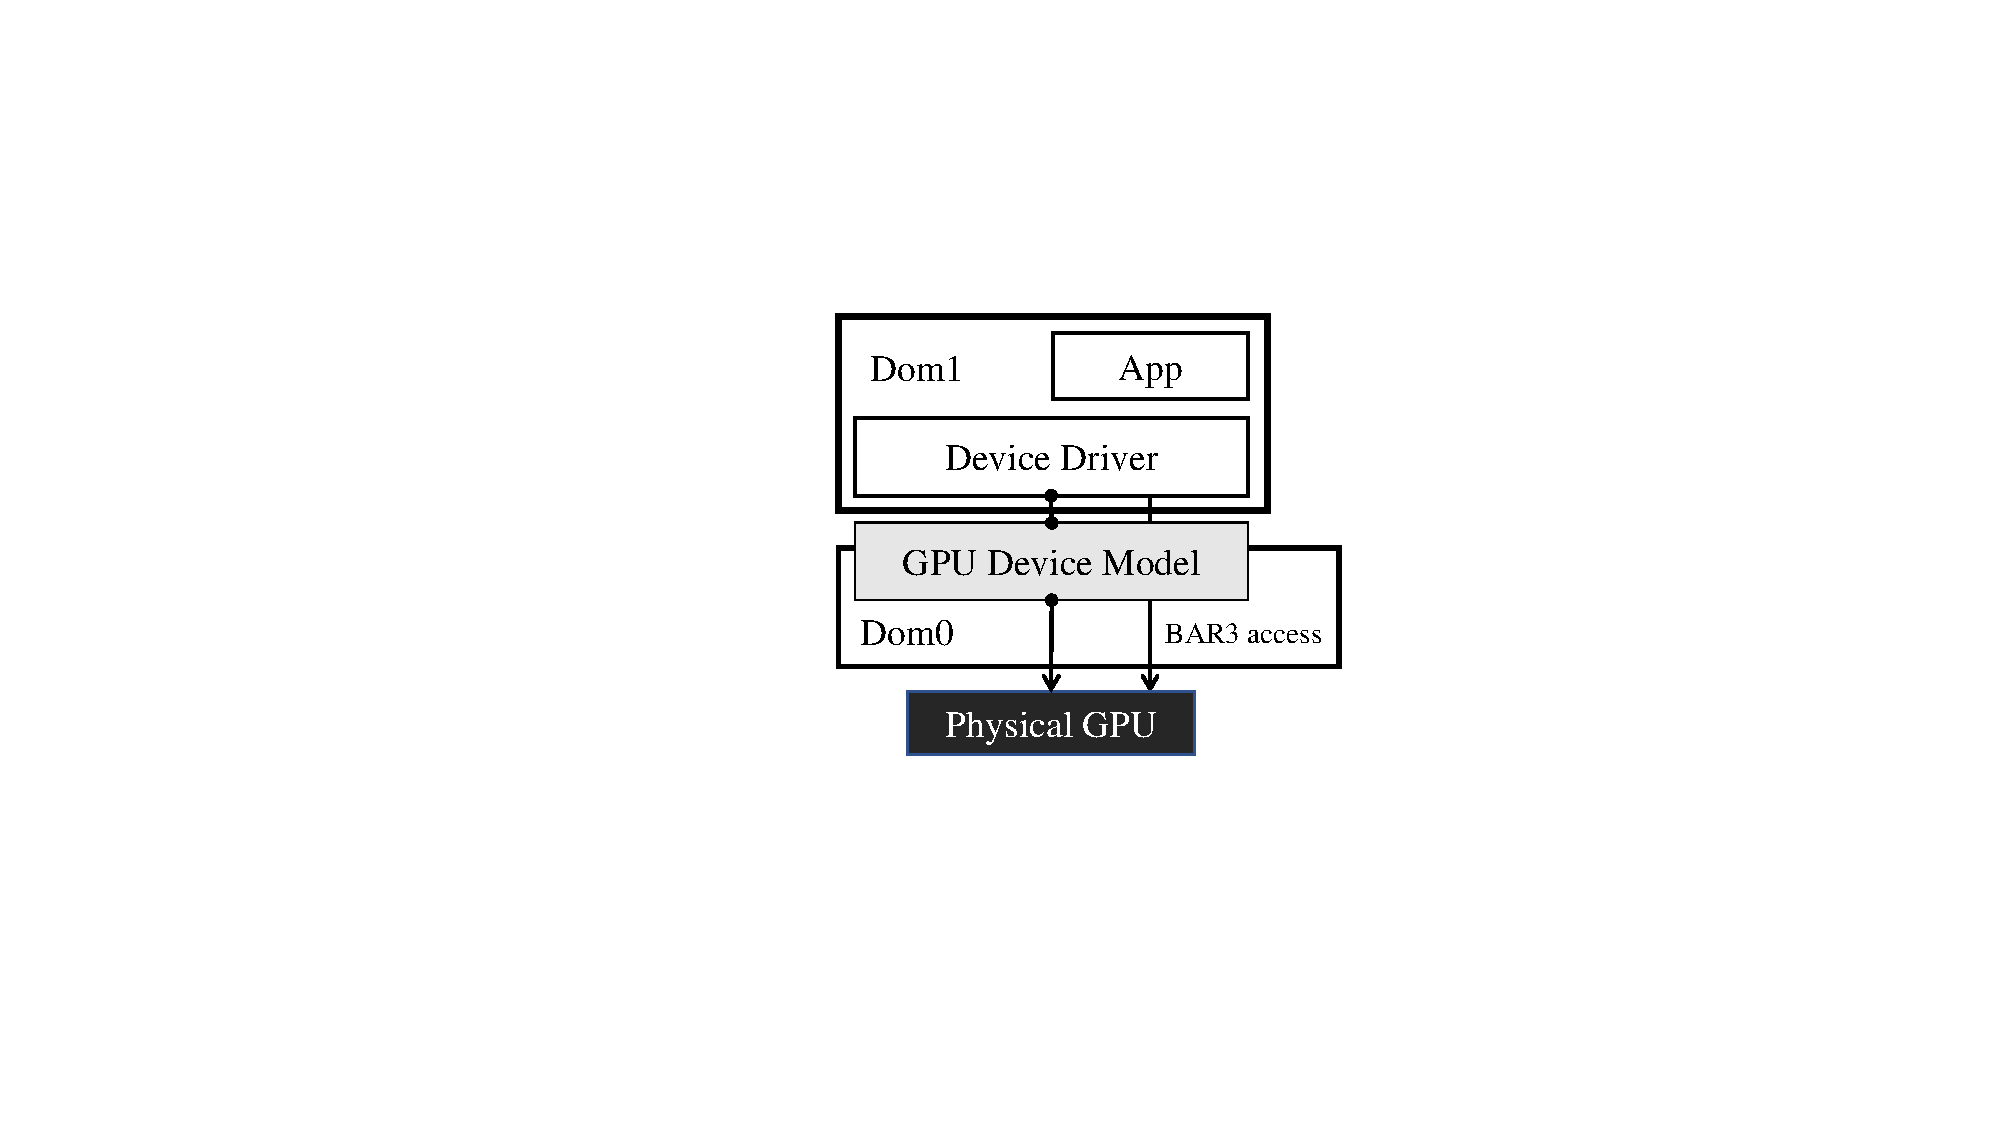
\includegraphics[width=.5\columnwidth,trim={14cm 6.2cm 11cm 5cm},clip]{images/gpuvm/gpuvm_basic.pdf}
	\caption{{\footnotesize Trap-based virtualization example: GPUvm. BARs, short for Base Address Registers, is exposed to PCIe and map the GPU control registers and  memory apertures.}}
	\label{fig_gpuvm_basic}
\end{figure}


\begin{figure}[!th]
	\centering
	\begin{subfigure}{.8\columnwidth}
		\centering
		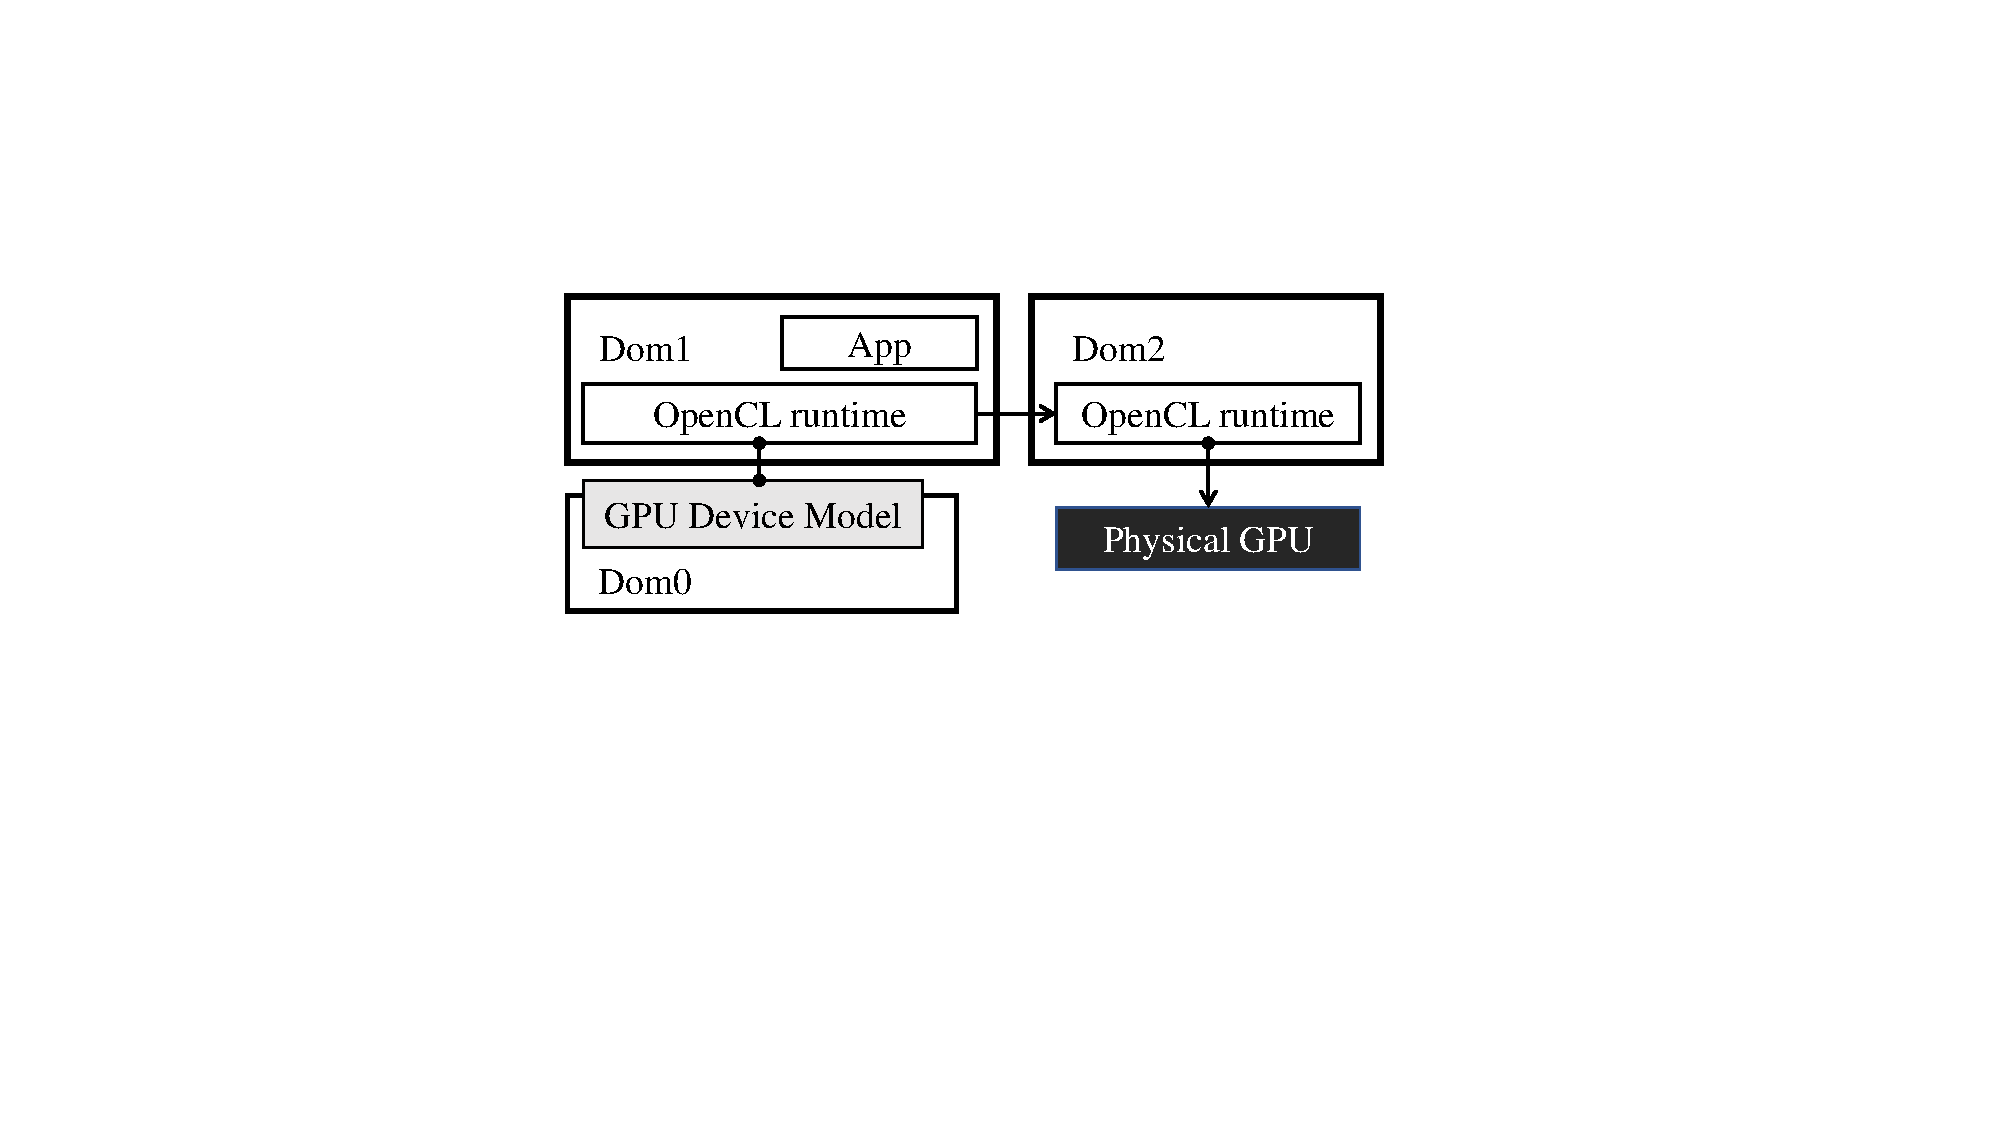
\includegraphics[width=\columnwidth,trim={9cm 8.5cm 10cm 4cm},clip]{images/gpuvm/gpuvm_api.pdf}
		\caption{{\footnotesize User-space API remoting over RPC --- executed on GPU.}}
		\label{fig_gpuvm_api}
	\end{subfigure}\hfill
	\begin{subfigure}{.75\columnwidth}
		\centering
		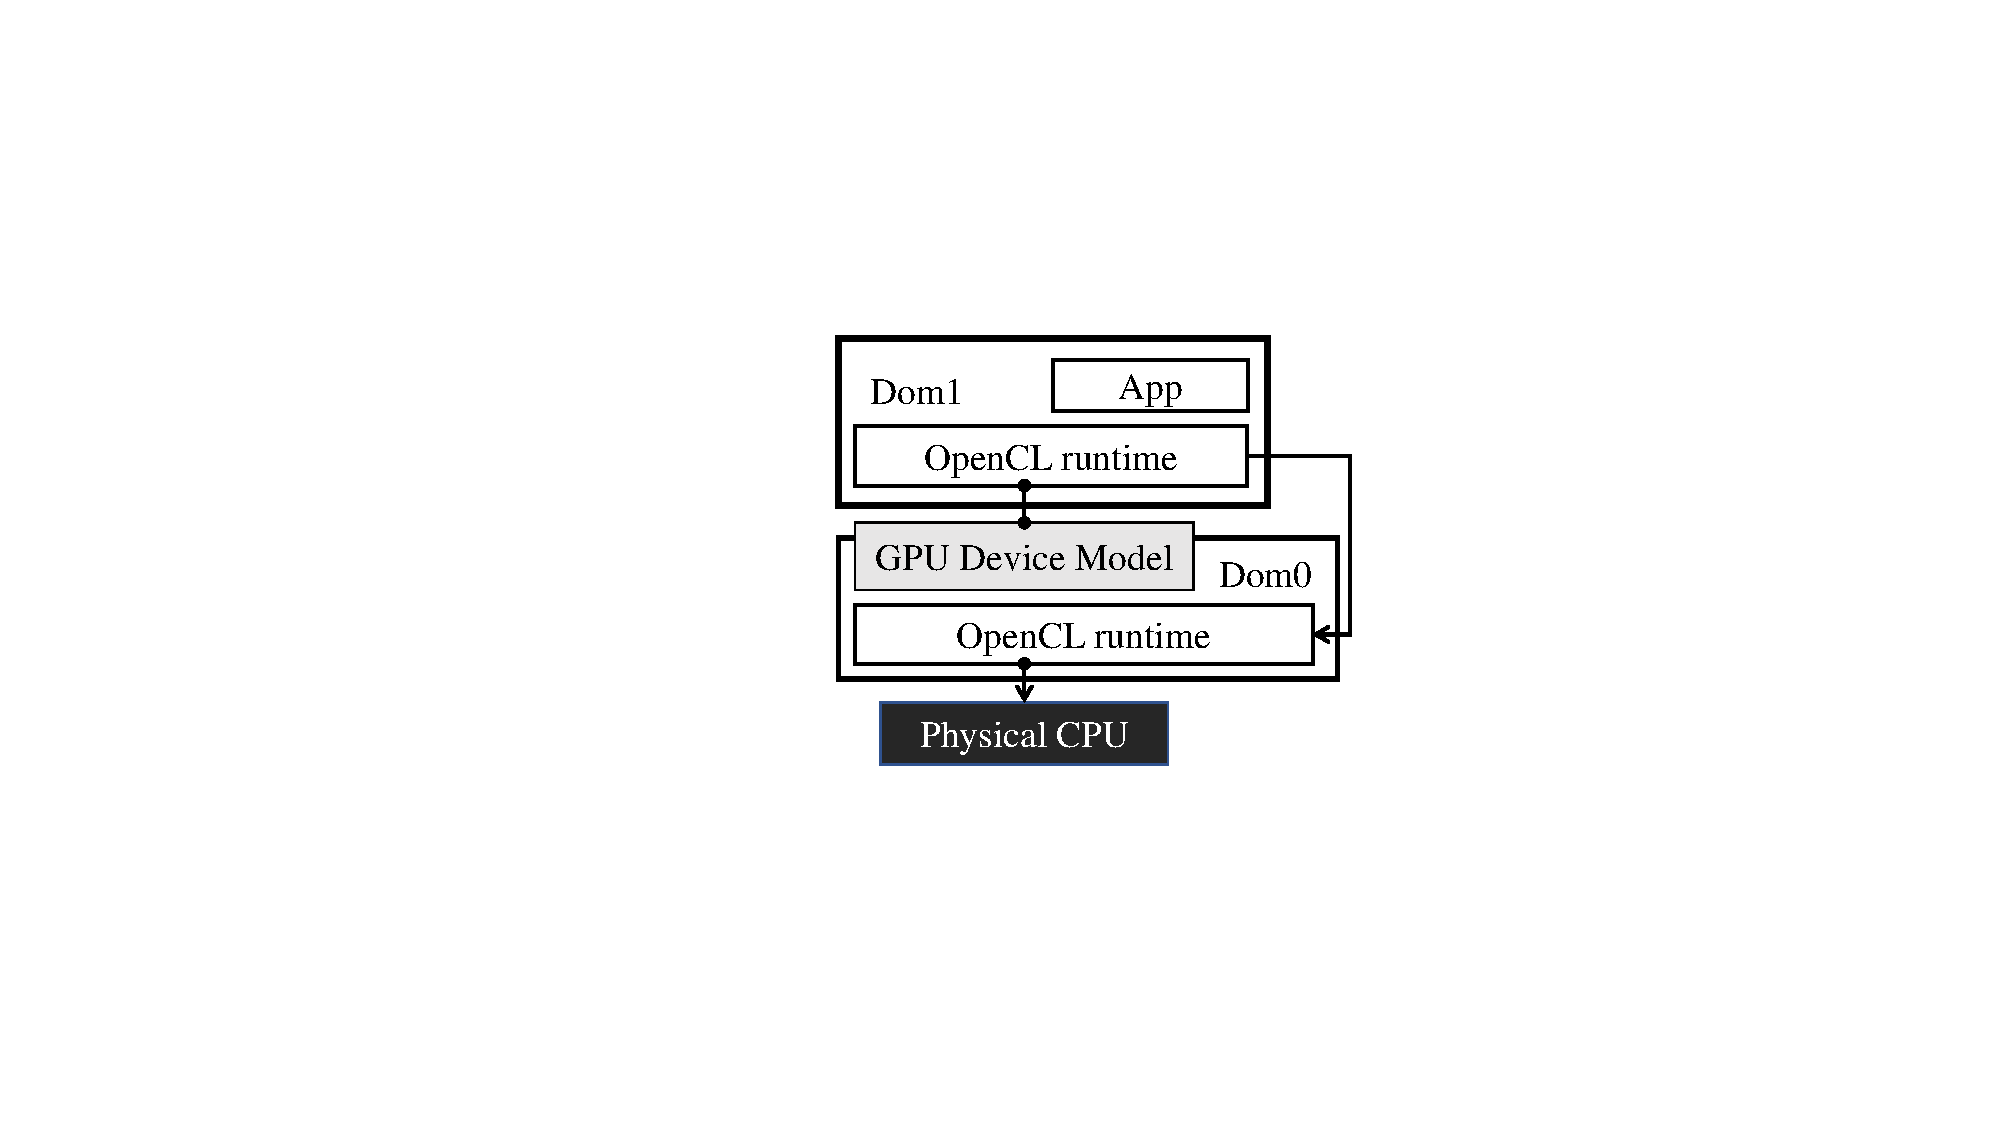
\includegraphics[width=.6\columnwidth,trim={14cm 6cm 11cm 5cm},clip]{images/gpuvm/gpuvm_cpu.pdf}
		\caption{{\footnotesize User-space API remoting over RPC --- executed on CPU.}}
		\label{fig_gpuvm_cpu}
	\end{subfigure}
	\caption{{\footnotesize API remoting examples: prototypes on Xen HVM. (a) API-remoting; (b) remote-emulation.}}
	\label{fig:api_remote}
\end{figure}
